\chapter{FlexTouch Implementation}

To validate the feasibility of our approach across different Android devices, We implemented \textit{FlexTouch} on a Huawei P20 and a Huawei P10 phone. By rooting the Android operating system and modifying the driver of the touch screen controller IC in the kernel's source code, we extracted the raw capacitive sensing data: $32 \times 16 = 512 px$ 16-bit diff value image across a 5.8-inch surface at 100 fps for Huawei P20 phone, $28 \times 16 = 448 px$, 16-bit diff value image across 5.1-inch surface area at 20 fps for Huawei P10 phone. We built an Android application that shows positions and raw capacitive values with corresponding update rates of chosen sensing nodes. The app also logs the raw capacitive image to a local server for later analysis.

\begin{figure}[ht]
    \centering
      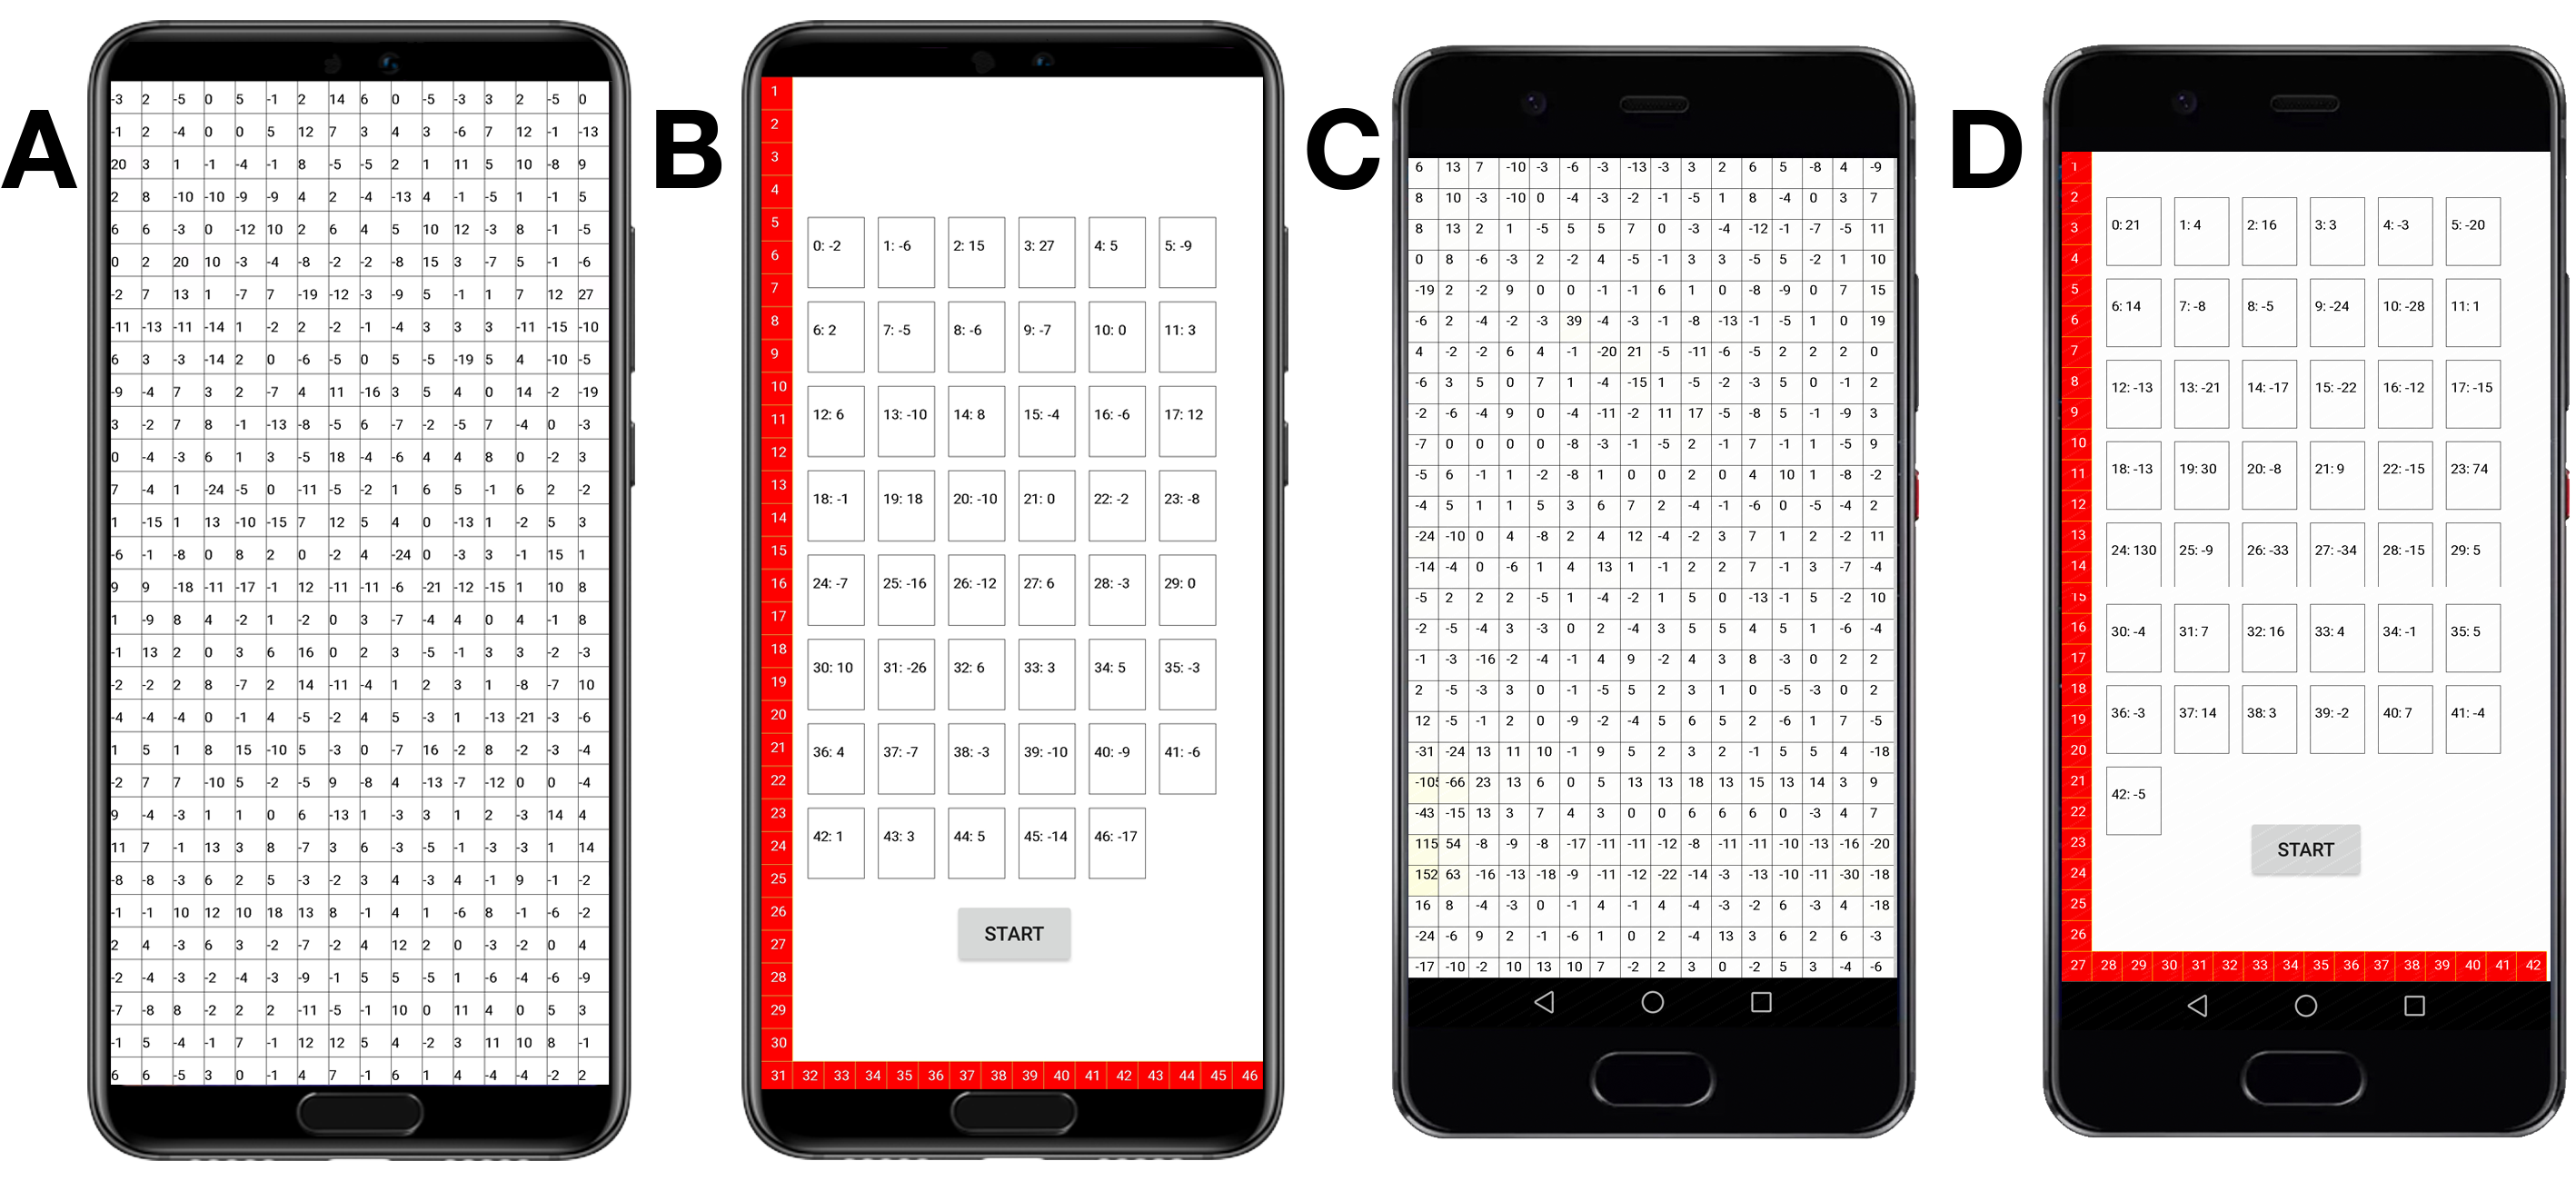
\includegraphics[width=0.95\columnwidth]{figures/rawdata.png}
      \setlength{\belowcaptionskip}{-6pt}
      \caption{Android Applications showing the raw capacitive data and positions of the sensing nodes.}
      \label{fig:Android Applications showing the raw capacitive data and positions of the sensing nodes.}
\end{figure}

\section{FlexTouch Sensing Capabilities}
We summarized the sensing capabilities of \textit{FlexTouch} into four categories as shown in Figure ~\ref{fig:1d2d-principle}. 

a) 1D touch interfaces enable tangible discrete touchable buttons, 1D touch gesture widgets.

b) 2D continuous multi-touch tracking enables large-scale multi-touch tracking or hand/body activity detection. 

c) 2D High resolution single-touch tracking via extending ($N$) capacitive sensing junctions into X-Y matrix configuration that enables $N^2/4$ capacitive sensing nodes. 

d) Everyday object state sensing includes object presence detection and object state sensing based on capacitance measurement. 

Note that sensing capability a) has been discussed in prior work ~\cite{Kato2015}. But the other modalities are unique to \textit{FlexTouch}.

\begin{figure}[h]
\centering
  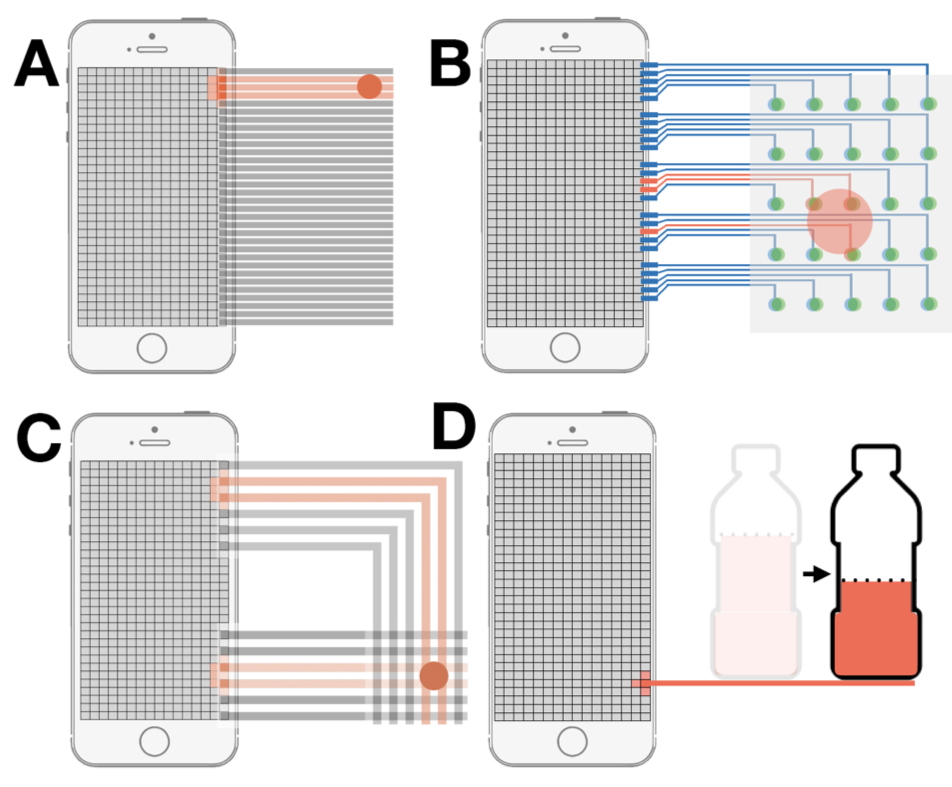
\includegraphics[width=0.95\columnwidth]{figures/1d2d-principle.png}
  \caption{\textit{FlexTouch} supports various applications with different sensing capabilities including A: 1D touch sensing, B:2D continuous multi-touch tracking, C: 2D High resolution single touch tracking and D: Object presence and state sensing}
  \label{fig:1d2d-principle}
\end{figure}

\section{Signal Processing for Touch Event Detection}
In this section, we use the P20 phone as an example to present the signal processing and the touch event detection pipeline of \textit{FlexTouch}. 

Fig ~\ref{fig:processing} demonstrates the signal processing procedure to detect the touch event on a 3-meter extension tape attached to the touchscreen. To filter out the high-frequency background noises, we applied a moving-average filter on the raw capacitive data using the unweighted mean of the previous 10 data points. During a touch event, a sharp signal rise occurs. To detect these rising step events, we applied a sliding window that contains 20 data points on a low-pass filtered signal. The step event can be extracted by comparing the data samples in front of the sliding window queue and at the tail of the queue. Each data sample in the black line graph in Fig ~\ref{fig:processing} is calculated using the following equation where $S_{i}$ represents the filtered capacitive data. 

\begin{equation}
    S_{diff} = \frac{S_{16} + S_{17} + S_{18} + S_{19}}{4}  - \frac{S_{0} + S_{1} + S_{2} + S_{3}}{4}
\end{equation}

Here we define the \textbf{\textit{signal-to-noise ratio (SNR)}} representing the signal strength of the raw capacitive data. As shown in Fig ~\ref{fig:processing}, we define the \textbf{\textit{Noise}} to be the difference between the maximum and minimum values of 100 data points for P20 before the touch event. The \textbf{\textit{Signal}} is the $S_{diff}$. To extract the touch signal from the background noise effectively, the SNR should be greater than a predetermined threshold. In theory, if SNR > 1, we can detect touch events. 

\begin{figure}[ht]
    \centering
      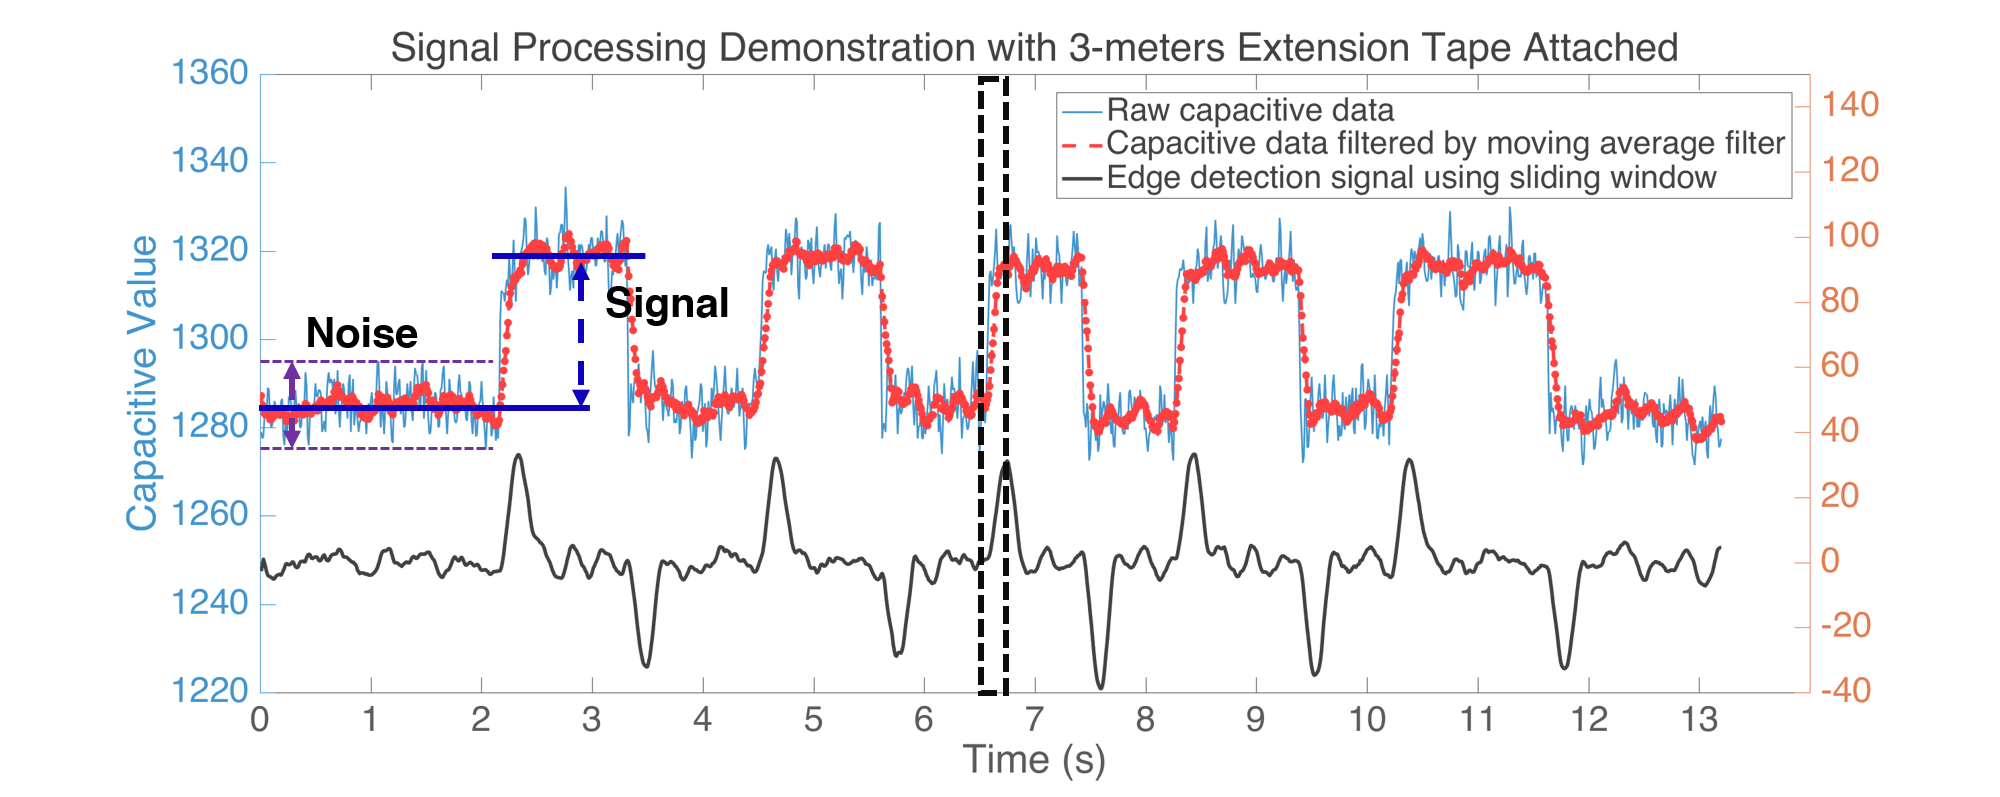
\includegraphics[width=0.95\columnwidth]{figures/processing.png}
      \setlength{\belowcaptionskip}{-8pt}
      \caption{Signal processing demo  detecting the touch event.}
      \label{fig:processing}
\end{figure}

\section{Differentiation Between On-screen and Off-screen Event}
% to be added tomorrow
% one figure 

\section{Fabrication}
We identified materials that can be easily customized into everyday surfaces with properties including flexibility, conductivity, and commercial availability. We fabricated interfaces using these materials through various processes, including adhering, cutting (e.g., manual cutting, laser cutting) and coating methods (e.g., ink-jet printing, brush painting). We leveraged the following materials to fabricate \textit{FlexTouch} interfaces.

\subsection{Conductive Tapes}
Conductive adhesive tapes are widely used for electromagnetic shielding and transmission wiring (e.g. paper circuits). The most widely available conductive tape is an adhesive copper foil tape that can be found at most hardware, electronic or gardening stores (Fig ~\ref{fig:material} A). It is \$2.50 per roll (6.3 mm x 20 m). The copper tape is highly conductive on both sides (0.05 $\Omega$ per square centimeter).

End-users can manually arrange any layout on any surface using copper foil tapes (e.g., Fig ~\ref{fig:material} E) without any additional fabrication equipment. In addition, the conductive tape is more flexible and suitable for large-scale applications since it can easily adhere to everyday objects. However, the copper foil tape is not suitable for volume production since it is not compatible with current fabricating techniques such as laser cutting or printing.

\begin{figure}
\centering
  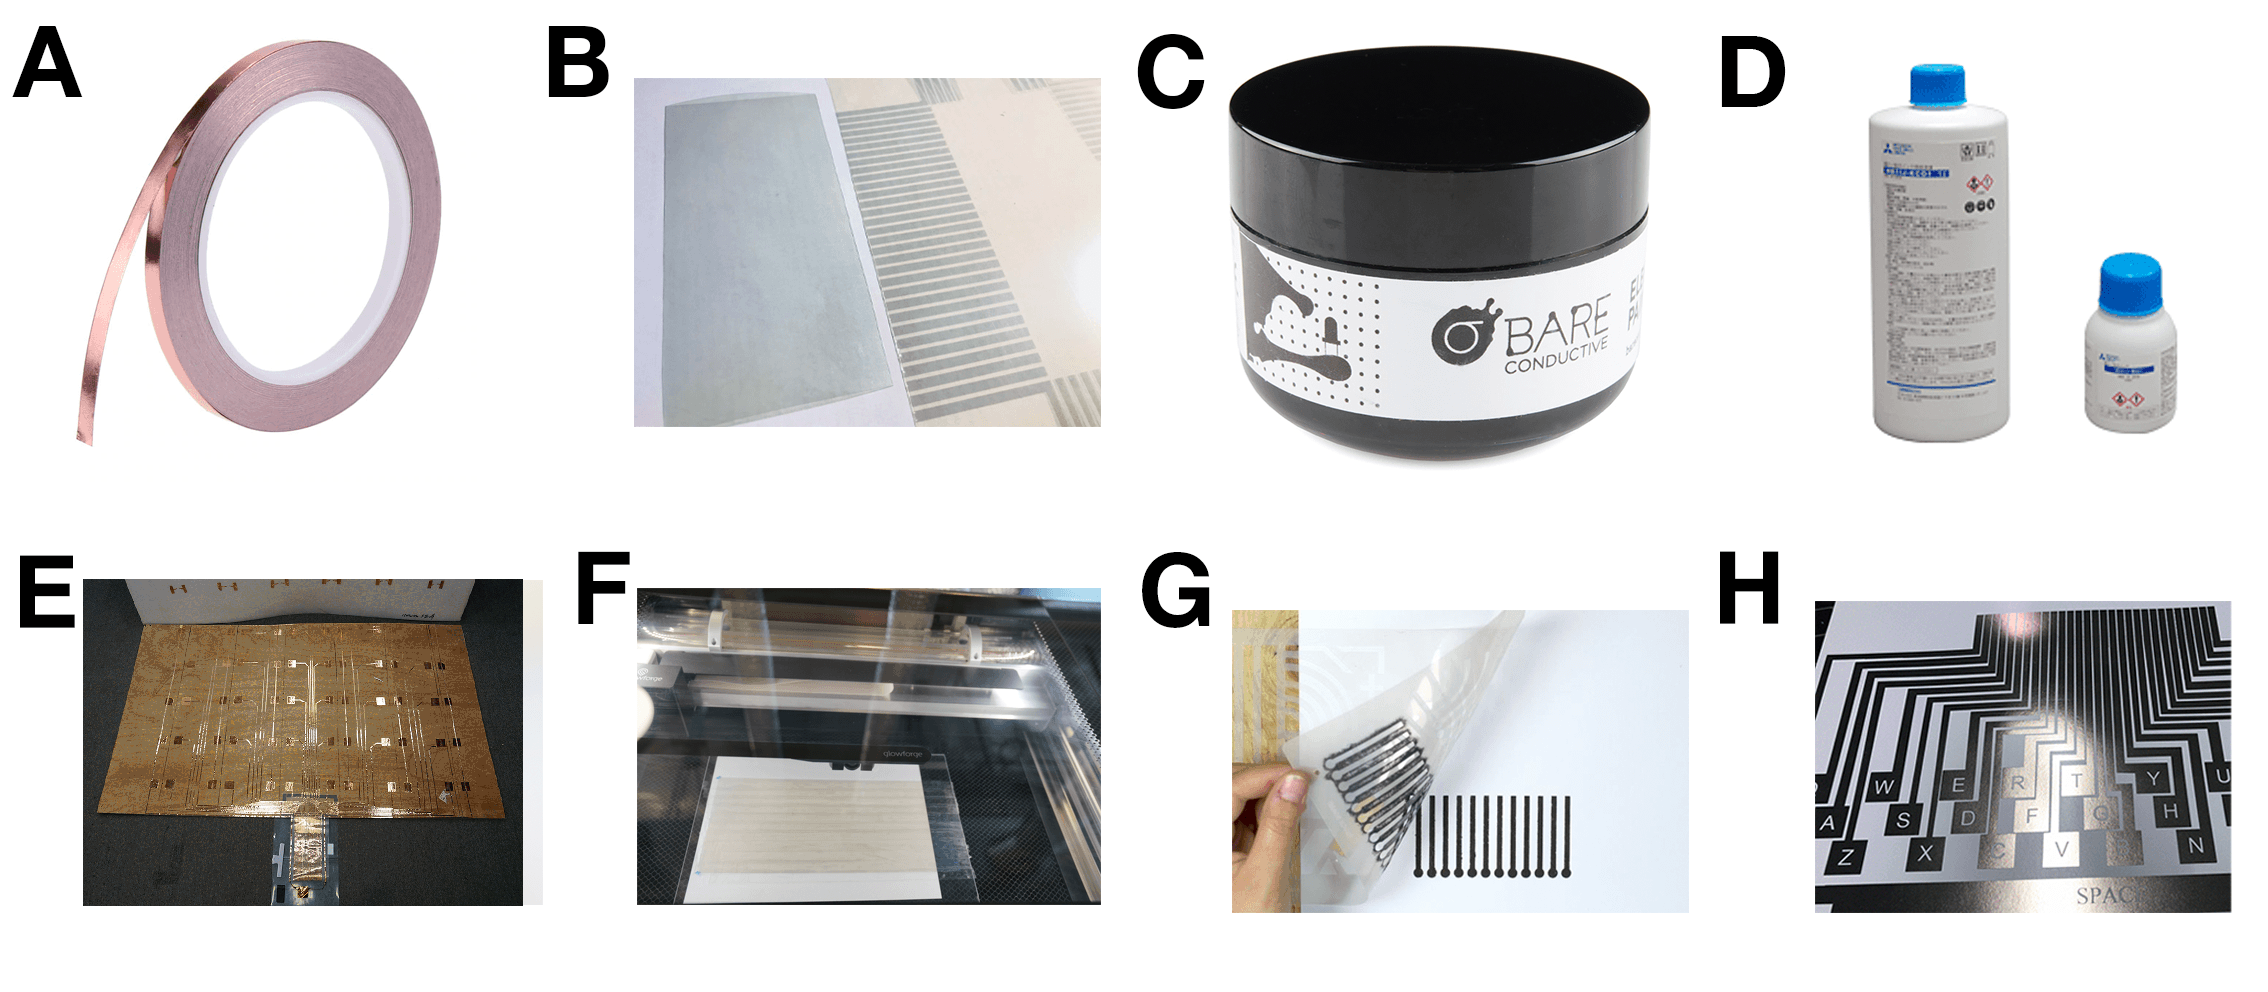
\includegraphics[width=0.95\columnwidth]{figures/material.png}
  \setlength{\belowcaptionskip}{-6pt}
  \caption{Commercially available materials. Copper foil tape (A) can be fixed to any surface (E). ITO PET Plastic film (B) can be fabricated to any 2D pattern using a laser cutter (F) or manually. Bare conductive carbon paint (C) and screen painting (G). Ink-jet circuit printer with Mitsubishi Silver nanoparticle ink (D) for printable conductive 2D layout (H). }
  \label{fig:material}
\end{figure}

\subsection{Conductive Films}
Film-like materials can be subtracted to 2D patterns using cutting or etching fabrication methods. One example material is the flexible Indium Tin Oxide (ITO) coated PET plastic film that is semi-transparent and conductive. We use the commercially available ITO-coated PET film manufactured by HNXCKJ ~\cite{ITO} that is compatible with laser cutters. Furthermore, 2D custom layouts are also available by coating ITO materials on extremely thin ($0.05 mm$) plastic film at a cost of \$30 per square foot (Fig ~\ref{fig:material} B).

Since the ITO-coated PET plastic film is highly transparent, it can be attached to the touchscreen without occluding the display (Fig ~\ref{fig:plugandplay} A). The ITO film can be customized as a screen protector for daily use with an array of ITO strips attached to the edges of the screen. This ITO strip array interface can be connected to the external application easily with a plug and play design as Fig \ref{fig:plugandplay} A and B show.

\subsection{Conductive Coating}
Liquid paint coating and ink printing are more versatile, as they can be added onto any surface in post-production. We identified two coating materials as examples. We use conductive carbon paint from Bare Conductive (Fig ~\ref{fig:material} C, \$280 per litter).  This material can be painted on a flat surface such as a wooden board or cardboard, and then laser cut to engrave the layout on top of it. Another suitable coating material is printable ink. We identified Silver nanoparticle ink made by Mitsubishi (Fig ~\ref{fig:material} D, \$340 per 100 ML) as presented by Instant Inkjet Circuits ~\cite{Kawahara-inkjet}. We fabricated the inkjet printable circuit with a Brother MFC-J480DW model printer. 

The conductive coating method is compatible with mass production due to its reproducibility. However, because of the limited size of each template or substrate, we need to further assemble the fabricated elements for large-scale application.

\section{Plug and Play}
In this section, we present \textit{FlexTouch}'s plug and play interface for daily use by proposing two assembly approaches as demonstrated in Fig ~\ref{fig:plugandplay}. 

\begin{figure}[ht]
    \centering
      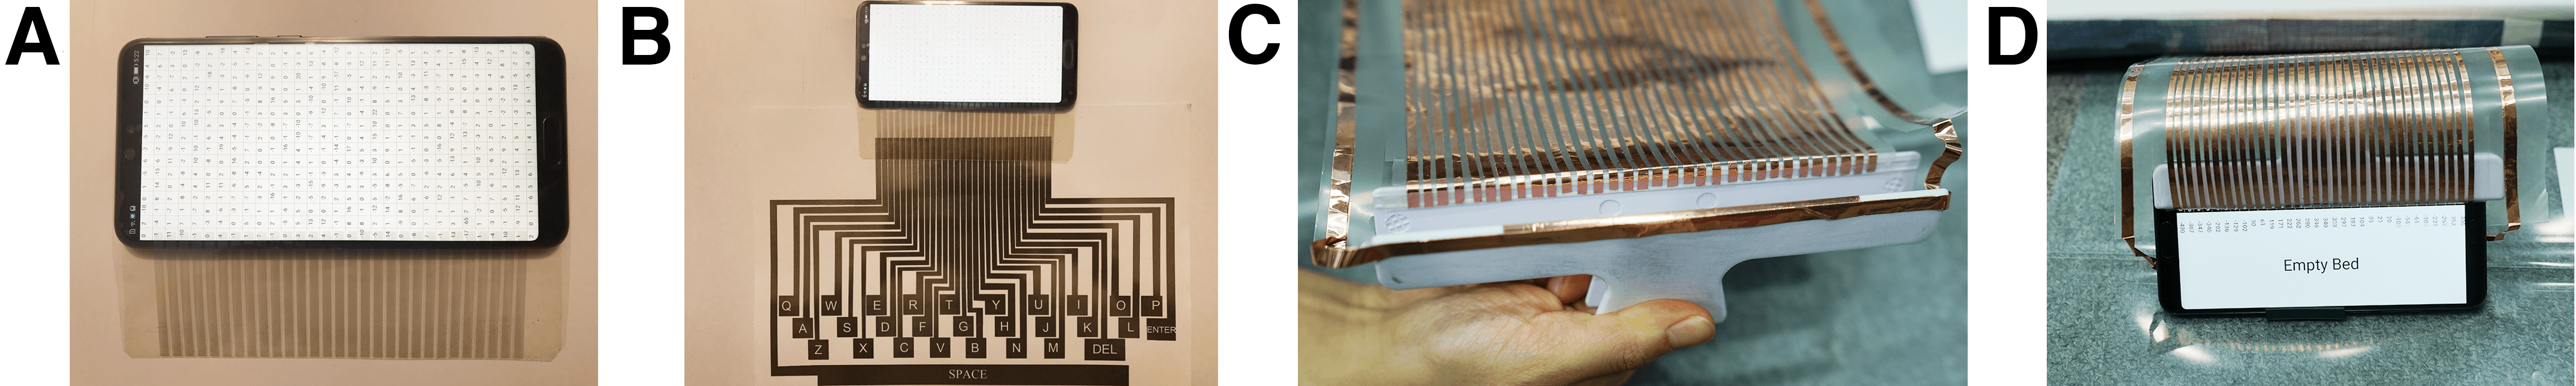
\includegraphics[width=0.75\columnwidth]{figures/plugandplay.png}
      \setlength{\belowcaptionskip}{-6pt}
      \caption{Demonstration of two assembly methods. The ITO strip array interface (A) can be stuck to a 2D-patterned application (B). The external application can be clipped onto the edge of the touchscreen (C and D).}
      \label{fig:plugandplay}
\end{figure}

\begin{itemize}
    \item \textbf{Adhere the external application with an ITO array film.} The ITO film is suitable for being integrated into a screen protector with an ITO conductive array connected to the edge of the touchscreen. The adhesive ITO film can easily be attached or detached to the external 2D patterned application. 
    \item \textbf{Fix the external application on the phone's edge with a clip.} The external application is connected with an array of conductive threads on one side of the clip while the electrodes on the 2D pattern representing the local ground are connected on the other side of the clip as shown in Fig ~\ref{fig:plugandplay} C. The customized part can be clipped onto the edge of the touchscreen as shown in Fig ~\ref{fig:plugandplay} D. 
\end{itemize}



